\section{Credit Capacity and Collateral Release}\label{sec:credit}

\Cref{lem:exact} gives the cash needed for redemptions at one state. A lending rule must also cover the states that borrowers can create by repaying. This section characterizes that requirement for a fixed curve. It then gives two ways of lending beyond the floor: commit an additional reserve, or change the collateral released by a repayment. The additional credit has a cost in each case. The first uses capital that cannot be skimmed; the second restricts withdrawal and splitting of positions. These are extensions of the model, not claims that its original floor bound is incorrect.

\subsection{Repayment rights and cash coverage}\label{cr:rights}

Fix a schedule $p$ and its reserve function $R$. There are finitely many loans $(\ell_i,d_i)$, with $\ell_i,d_i>0$, total lock $L\le S$, and cash $A\ge0$. Custody holds, and $W=A+D-R(S)\ge0$. We allow debts above the floor, so (J2) is \emph{not} assumed. Initially consider only repayments and redemptions at their full gross curve return. There is no new borrowing, minting, reshaping, accrual, reserve withdrawal or fee retention. Thus $W$ is constant. Borrowers may supply the cash needed to repay; safety is required for all allowed repayment choices, whether or not those choices maximize their payoffs.

For each loan, let $\mathcal E_i\subseteq[0,\ell_i]\times[0,d_i]$ be the closure of the set of residual pairs $(q_i,b_i)$, locked tokens and remaining debt, attainable by a finite sequence of repayments. It includes the initial pair and $(0,0)$. Repayment rights are local to the loan: they do not depend on other loans, free balances or redemptions. Each combination of attainable pairs can therefore be reached by making the loans' repayments in turn, before any redemption. Taking the closure includes limits of such combinations; the cash inequalities below are continuous and are unchanged by this convention. Full repayment releases the whole lock. We call a state \emph{safe under its repayment rights} if every finite sequence of these repayments and gross redemptions can be executed without a cash shortfall.

\begin{theorem}[Coverage under repayment rights]\label{cr:kernel}
The state is safe under its repayment rights if and only if
\begin{equation}\label{cr:allpairs}
\sum_i b_i\;\le\;W+R\!\left(\sum_i q_i\right)
\qquad\text{for every }(q_i,b_i)\in\mathcal E_i\text{ for all }i.
\end{equation}
When $W=0$, this is equivalent to the separate conditions
\begin{equation}\label{cr:individual}
b\le R(q)\qquad\text{for every }(q,b)\in\mathcal E_i\text{ and every }i.
\end{equation}
\end{theorem}
\begin{proof}
After any repayments and redemptions, write $S',D',L',A'$ for the current state. Repayments preserve $A+D$, and a gross redemption reduces $A$ and $R(S)$ by the same amount. Thus $A'+D'-R(S')=W$. Redeeming all free tokens would leave cash
\[
A'-[R(S')-R(L')]=W+R(L')-D'.
\]
If \eqref{cr:allpairs} holds, that cash is non-negative at every possible loan state; every smaller redemption can also be paid. Repayments add cash. Conversely, a violation at an attainable residual configuration is exposed by making those repayments and then redeeming all free tokens. A strict violation at a limit configuration is also a violation at a nearby attainable one.

For the last claim, convexity and $R(0)=0$ give
\begin{equation}\label{cr:superadd}
\sum_i R(q_i)\le R\!\left(\sum_iq_i\right).
\end{equation}
Indeed $R(q_i)\le q_i R(Q)/Q$ for $Q=\sum_iq_i>0$. Hence \eqref{cr:individual} suffices. It is necessary because all loans other than $i$ can be fully repaid, leaving their residual pairs equal to $(0,0)$.
\end{proof}

For any repayment rights we write $W_{\min}$ for the least reserve that satisfies \eqref{cr:allpairs}: the supremum of $\sum_ib_i-R(\sum_iq_i)$ over attainable configurations, which is at least zero. \Cref{cr:buffer} computes it for proportional release.

The quantifier over future repayments is essential. For $R(q)=q+q^2/2$, a one-token lock against debt $3/2$ satisfies the current condition $D=R(L)$. If $S=L=1$ and $W=0$, cash is zero. Repaying $3/4$ and releasing half the collateral makes $3/4$ cash available, but redeeming the released half costs $R(1)-R(1/2)=7/8$. The shortfall is $1/8$. No price movement or other borrower is needed.

\subsection{Proportional release and the committed reserve}\label{cr:proportional}\label{sec:credit-buffer}

Under proportional release, $\mathcal E_i=\{(x\ell_i,xd_i):0\le x\le1\}$. Put $a_i=d_i/\ell_i$. For $0\le q\le L$, define
\begin{equation}\label{cr:envelope}
H(q)=\max\left\{\sum_i a_iq_i:
0\le q_i\le\ell_i,\ \sum_iq_i=q\right\}.
\end{equation}
This is the fractional-knapsack envelope: retain collateral from loans with the largest $a_i$ first \citep{kellerer2004}. It is continuous, concave and piecewise linear. For $L>0$, if $Z$ takes value $a_i$ with probability $\ell_i/L$, then $H(q)=L\int_{1-q/L}^{1}F_Z^{-1}(u)\,du$, an upper integrated-quantile function \citep{gushchin2017}. For an empty book, set $H(0)=W_{\min}=0$. The sorting argument is classical; its role here is to identify the residual loan book that places the greatest demand on cash.

\begin{theorem}[Exact buffer for proportional release]\label{cr:buffer}
With proportional release, the least non-negative committed reserve required by \cref{cr:kernel} is
\begin{equation}\label{cr:wmin}
W_{\min}=\max_{0\le q\le L}\{H(q)-R(q)\}.
\end{equation}
In particular, when $W=0$, safety under all repayment choices holds if and only if $d_i\le\Pf\ell_i$ for every loan. This necessity applies to heterogeneous and state-dependent loan allocations, not only to a uniform cap.
\end{theorem}
\begin{proof}
At fixed residual total $q$, \eqref{cr:envelope} is the largest possible remaining debt. Substitution in \cref{cr:kernel} gives \eqref{cr:wmin}; its maximum is at least zero because $H(0)=R(0)=0$. For $W=0$, \eqref{cr:individual} requires $xd_i\le R(x\ell_i)$ for every $x>0$. Divide by $x\ell_i$ and let $x$ decrease to zero to obtain $a_i\le\Pf$. Conversely, $a_iq_i\le\Pf q_i\le R(q_i)$, so \eqref{cr:individual} holds.
\end{proof}

For a uniform cap per token, the necessity of the floor bound is \cref{prop:tight}. The statement here extends it in two ways: it holds loan by loan for any allocation of debt, and it follows from the repayment rights alone, without constructing a sequence of borrowing operations.

The function $H-R$ is concave. Its maximum is found where the non-increasing slope of $H$ crosses the non-decreasing price $p$, including endpoints and jumps. Sorting the ratios takes $O(n\log n)$ comparisons. With rational stepped or piecewise-affine prices, a scan of the price and collateral breakpoints finds the maximum exactly. \Cref{cr:algorithm} gives the representation and algorithm; an arbitrary price function instead requires an evaluation or optimization oracle.

\paragraph{Keeping the reserve committed.}
For this extended design, $W$ is not all available for withdrawal. The safe skim guard is $w\le W-W_{\min}$. A repayment restricts the remaining possible residual configurations, so it cannot increase $W_{\min}$ at a fixed curve. Gross sales leave both $W$ and the loan book unchanged; retaining fees can only increase $W$. New lending may be admitted by checking $W'\ge W_{\min}'$ in the resulting state. That test also implies $A'\ge0$, since the initial residual configuration gives $D'\le W'+R(L')\le W'+R(S')$. A reshape needs the same test with the new reserve function and the repayment rights that will remain in force. These are guards for a different mechanism; the original \op{Skim} guard in \cref{sec:model} must not be used with above-floor proportional loans. Full derivations are in \cref{cr:guards}.

\subsection{Allocation of a fixed reserve}\label{cr:allocation}

\begin{proposition}[Equal ratios and aggregate capacity]\label{cr:capacity}
Fix positive lock sizes with total $L>0$. Among allocations with total debt $D$, assigning $d_i=(D/L)\ell_i$ minimizes $W_{\min}$, weakly. The greatest aggregate debt consistent with proportional release and a committed reserve $W\ge0$ is
\begin{equation}\label{cr:dmax}
D_{\max}=L\inf_{0<q\le L}\frac{R(q)+W}{q}.
\end{equation}
An allocation with equal ratios attains this bound.
\end{proposition}
\begin{proof}
Concavity, $H(0)=0$ and $H(L)=D$ imply $H(q)\ge Dq/L$. Equal ratios attain equality at every $q$, so they weakly minimize \eqref{cr:wmin}. For that allocation, the safety constraints are $(D/L)q\le R(q)+W$ for every $q>0$, which are equivalent to \eqref{cr:dmax}. The infimum is finite and the corresponding constant ratio satisfies every constraint, whether or not the infimum is attained at a positive $q$.
\end{proof}

The minimizer need not be unique. This is a chord comparison for the classical envelope, rather than a new general optimization method. Its implication for credit is that two books with identical supply and total debt can require different reserves. With $R(q)=q+q^2/2$, $L=1$ and $D=3/2$, an equal ratio of $3/2$ requires $W_{\min}=1/8$. Two locks of $1/2$ with debts $1$ and $1/2$ require $W_{\min}=3/8$: the highest ratio is retained while the other loan is repaid. The reserve requirement triples although aggregate utilization is unchanged.

\begin{figure}[t]
\centering
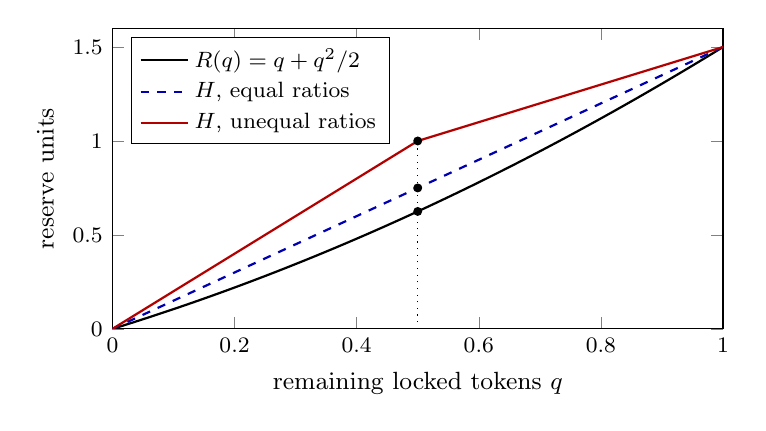
\begin{tikzpicture}
\begin{axis}[width=0.77\textwidth,height=5.4cm,
  xlabel={remaining locked tokens $q$},ylabel={reserve units},
  xmin=0,xmax=1,ymin=0,ymax=1.6,
  legend pos=north west,legend cell align=left,
  tick label style={font=\footnotesize},label style={font=\small},
  legend style={font=\footnotesize}]
\addplot[thick,black,domain=0:1,samples=101] {x+x*x/2};
\addlegendentry{$R(q)=q+q^2/2$}
\addplot[thick,dashed,blue!70!black,domain=0:1,samples=2] {1.5*x};
\addlegendentry{$H$, equal ratios}
\addplot[thick,red!70!black] coordinates {(0,0) (0.5,1) (1,1.5)};
\addlegendentry{$H$, unequal ratios}
\draw[thin,dotted] (axis cs:0.5,0) -- (axis cs:0.5,1);
\addplot[only marks,mark=*,mark size=1.4pt,black]
  coordinates {(0.5,0.625) (0.5,0.75) (0.5,1)};
\end{axis}
\end{tikzpicture}
\caption{The required reserve is the greatest vertical distance from $R$ to the debt envelope $H$. Both books have $L=1$ and $D=3/2$. Their maximum gaps occur at $q=1/2$ and are $1/8$ for equal ratios and $3/8$ for the two unequal ratios. These quantities are checked in script block CF01.}\label{cr:figure}
\end{figure}

For the linear price $p(q)=P+kq$, with $P>0$ and $k>0$, minimizing \eqref{cr:dmax} gives
\begin{equation}\label{cr:linearcapacity}
\frac{D_{\max}}L=
\begin{cases}
P, & W=0,\\[2pt]
P+\sqrt{2kW}, & 0<W\le kL^2/2,\\[2pt]
P+kL/2+W/L, & W>kL^2/2.
\end{cases}
\end{equation}
The interior minimizing depth is $\sqrt{2W/k}$. The formula describes cash coverage, not a positive residual for every borrower. An above-floor proportional loan can become worth less than its debt after a partial repayment, even when the committed reserve makes every free redemption payable. For example, in the one-token case above, $W=1/8$ pays the released half, but the remaining debt $3/4$ exceeds $R(1/2)=5/8$. A collateral-funded close is a separate requirement.

\paragraph{Cash coverage is not an incentive to repay.}
The buffer makes above-floor loans payable; it does not make them worth repaying, and the incentive results of \cref{sec:incentives} do not carry over. For exit routing, a holder whose tokens would redeem for a gross value $v$ per token receives $(1-f_s)v$ by redeeming and $(1-\phi)a$ by borrowing at the ratio $a$ and never repaying. Abandonment pays whenever $(1-\phi)\,a>(1-f_s)\,v$, the condition of \cref{prop:route} with $\gamma\Pf$ replaced by $a$. For a holder who redeems at the floor, $v=\Pf$, and a ratio $a>\Pf$ satisfies the condition unless the fees are at least as large as the lending premium, $(1-f_s)/(1-\phi)\ge a/\Pf$. The rule $\gbar+\fsbar<1$ guaranteed the opposite inequality at every fee within the cap; lending above the floor removes that guarantee.

Borrowers can do better than choose between repaying in full and abandoning. They can repay in part, redeem the collateral that the repayment releases, and abandon the rest. The next result says exactly how much this takes out.

\begin{proposition}[What a committed reserve can lose]\label{cr:extraction}
In the setting of \cref{cr:rights}, with no fees, let the book be safe under its repayment rights, that is, $W\ge W_{\min}$. Let a coalition hold all $L=S$ tokens, locked against the loans of the book, and let the reserve $W$ have been paid in by someone else.
\begin{enumerate}[label=(\alph*)]
\item If the coalition repays down to an attainable residual configuration with total lock $Q$ and total debt $B$, redeems the released tokens and never repays the rest, it receives $B-R(Q)$ more than by repaying every loan and redeeming every token. The supremum of this gain over attainable configurations, which is the maximum over their closure, is $W_{\min}$, the least reserve that \cref{cr:kernel} requires. Under proportional release the supremum is attained.
\item After a path that attains this maximum the issuer holds cash $W-W_{\min}$.
\item Under proportional release, a book that is admitted with total debt $D_{\max}$ of \eqref{cr:dmax} and $W>0$ has $W_{\min}=W$: the coalition can take the whole reserve.
\item For a coalition that buys the $L$ tokens from an empty curve and pays a buy fee $f_b$, an origination fee $\phi$ and a sell fee $f_s$, all proportional and paid out of the mechanism, the profit of the path in (a) is
\[
\Pi=B-R(Q)-f_b\,R(L)-\phi\,D-f_s\,\bigl[R(L)-R(Q)\bigr].
\]
\item Under the curve-valued contract of \cref{cr:nonlinear} every attainable configuration has $B\le R(Q)$, so the gain in (a) is never positive.
\end{enumerate}
\end{proposition}
\begin{proof}
Because the book is safe under its repayment rights, every repayment and redemption below can be executed; without that hypothesis $B-R(Q)$ is still the difference of the two cash flows as written, but the issuer may run out of cash before the redemption is paid. (a) Repaying down to the configuration costs $D-B$ and the released $L-Q$ tokens redeem for $R(L)-R(Q)$; repaying everything costs $D$ and returns $R(L)$. The difference is $B-R(Q)$. By \cref{cr:kernel} the least admissible reserve is the supremum of $\sum_ib_i-R(\sum_iq_i)$ over attainable configurations, equivalently its maximum over their closure, and it is at least zero because $(0,0)$ is attainable for every loan. (b) The proof of \cref{cr:kernel} gives the cash after the path as $W+R(Q)-B$. (c) Because $W>0$, the function $(R(q)+W)/q$ tends to infinity as $q\downarrow0$ and is continuous on $(0,L]$, so the infimum in \eqref{cr:dmax} is attained at some $q^\ast>0$, where $(D_{\max}/L)\,q^\ast=R(q^\ast)+W$. By concavity $H(q^\ast)\ge D_{\max}q^\ast/L$, so $H(q^\ast)-R(q^\ast)\ge W$, and admission requires $W_{\min}\le W$. (d) The purchase costs $(1+f_b)R(L)$, the loans pay out $(1-\phi)D$, the repayment costs $D-B$ and the redemption returns $(1-f_s)[R(L)-R(Q)]$; the sum is $\Pi$. (e) The persistent condition \eqref{cr:nonlinearcover} holds at every attainable configuration, so $B\le\gbar\sum_iR(q_i)\le R(Q)$ by \eqref{cr:superadd}.
\end{proof}

The reserve that makes a proportional book safe is thus exactly the amount that a coalition of its borrowers can extract from it. Take $R(q)=q+q^2/2$, $L=S=1$ and $W=0.08$, which is below the threshold $kL^2/8=0.125$ at which $D_{\max}$ passes the redemption value $R(L)$ of the whole collateral. Then $D_{\max}=1.4<R(1)=1.5$, so repaying in full is still better than abandoning in full. But buying the token for $1.5$, borrowing $1.4$, repaying $0.84$ to release $0.6$ tokens, redeeming them for $1.02$ and leaving $0.4$ tokens locked against a debt of $0.56$ nets $0.08$: the whole reserve. The issuer is left with no cash and a residual loan of $0.56$ against collateral that redeems for $R(0.4)=0.48$: the loan is under-collateralized, in a state that remains safe under its repayment rights. With all three fees at $1\%$ the profit is $0.0408$ (script block N16). The statement is about a strategy that is available, under the stated assumptions on access and on who funded the reserve; it is not a prediction of what borrowers do, and a borrower who paid in the reserve counts that payment as a cost. The borrower's position is the residual claim of the corporate-debt model, the right to recover the collateral by paying the debt or to walk away \citep{merton1974}, and $W_{\min}$ is capital held against the worst admissible scenario, in the spirit of, though not shown to satisfy the axioms of, a coherent risk measure \citep{artzner1999}.

Two consequences follow. At the maximum admitted credit \eqref{cr:dmax}, the committed reserve is exposed to complete loss under the strategy above: it is first-loss capital for that path, though other repayment paths return it. And the amount that must stay committed is the current $W_{\min}$, not $W$: a repayment narrows the set of residual configurations and can lower the requirement, after which the difference may be withdrawn while the loan is open. In the example, repaying $1.12$ leaves $0.2$ tokens against a debt of $0.28$ and a requirement of $0.06$, so $0.02$ of the reserve is free. A path that repays and abandons can instead use up the cash and leave the remaining requirement committed for good. The curve-valued contract below does not have the defect, by part~(e), and under $\gbar+\fsbar<1$ redeeming a lock pays more than abandoning it.

\subsection{More credit with a different release rule}\label{cr:nonlinear}\label{sec:credit-release}

There is also a way to use the curve premium without an additional committed reserve. Suppose a partial repayment reduces debt but releases no collateral until the loan is fully repaid. By \cref{cr:kernel}, with $W=0$ such a book is safe under all repayments if and only if
\begin{equation}\label{cr:fullrelease}
d_i\le R(\ell_i)\qquad\text{for every loan}.
\end{equation}
Each remaining debt is at most its initial debt at the unchanged lock, and fully repaid loans disappear. Thus \eqref{cr:fullrelease} is the largest per-loan cap compatible with these rights and with the possibility that every other borrower exits.

Partial collateral release is possible if its amount is changed. Consider the operations of \cref{sec:model}, with the following replacements. The persistent loan condition is
\begin{equation}\label{cr:nonlinearcover}
d_i\le\gbar R(\ell_i),\qquad 0<\gbar\le1.
\end{equation}
A borrow is guarded by $d_i+b\le\gamma R(\ell_i+\ell^+)$, with $0<\gamma\le\gbar$. A partial repayment of $r$ may release $u\in[0,\ell_i]$ only if $d_i-r\le\gbar R(\ell_i-u)$; full repayment releases the whole lock. A reshape preserves \eqref{cr:nonlinearcover} for every loan under the new $R$, as well as satisfying (G1) and (G2). Custody, the definitions of $A,D,W$, and the remaining operations are unchanged. The release rule and the debt anchor are both different from those of the original model.

\begin{proposition}[Safety with a curve-valued lock]\label{cr:nonlinearsafety}
These operations preserve custody, \eqref{cr:nonlinearcover} and $A+D\ge R(S)$. Every free-token gross redemption and every admitted loan can be paid in full, without any repayment by another borrower. If proportional sell fees satisfy $f_s\le\fsbar$ and $\gbar+\fsbar\le1$, every loan can also be closed from its own collateral. The close leaves a positive residual when $\gbar+\fsbar<1$.
\end{proposition}
\begin{proof}
By \eqref{cr:superadd}, $D\le\gbar\sum_iR(\ell_i)\le\gbar R(L)$. This is the aggregate bound used in the coverage and cash-payout steps of \cref{thm:safety}. The modified borrow, repayment and reshape guards preserve the new individual condition; the other induction steps are unchanged. In particular a borrow gives $D+b\le\gbar R(S)$, so $A-b\ge(1-\gbar)R(S)$. For a close, monotonicity of $p$ gives
\[
R(S)-R(S-\ell_i)\ge R(\ell_i),
\]
and net proceeds are therefore at least $(1-\fsbar)R(\ell_i)\ge d_i$. Use the atomic netting of \cref{prop:netclose}. If $G=R(S)-R(S-\ell_i)$ is the gross return, the combined reserve outflow is at most $G-d_i$, and
\[
A-(G-d_i)=W+R(S-\ell_i)-(D-d_i)\ge0,
\]
because the other locks total at most $S-\ell_i$ and satisfy \eqref{cr:superadd}. With a strict inequality between the caps, the borrower's residual is at least $(1-\fsbar-\gbar)R(\ell_i)>0$.
\end{proof}

Since $R$ is strictly increasing, the largest release allowed by the new repayment guard is
\begin{equation}\label{cr:maxrelease}
u_{\max}(r)=\ell_i-R^{-1}\!\left(\frac{d_i-r}{\gbar}\right).
\end{equation}
At a loan's limit $d_i=\gbar R(\ell_i)$, convexity implies $u_{\max}(r)\le\ell_i r/d_i$. Paying half the debt therefore need not release half the tokens. In the preceding example with $\gbar=1$, repaying $3/4$ releases $2-\sqrt{5/2}\simeq0.418861$ tokens, whose curve return is exactly $3/4$. An integer implementation must round the remaining required lock upward; this section's result is real-valued, not a verification of such an implementation.

\paragraph{The stronger reshape guard matters.}
Let $p(q)=1+q$, $S=2$, one token locked against $d=3/2$, one token free, and $A=5/2$. Replace the curve by prices $1$ on $[0,1)$ and $3$ on $[1,2)$. The floor remains $1$ and total reserve remains $R(2)=4$, so (G1) and (G2) hold. But the new $R(1)=1$ no longer covers the loan, and the free token's return $3$ exceeds cash. Requiring $d_i\le\gbar R_{p'}(\ell_i)$ rejects this change. A sufficient condition that avoids inspecting each loan is $R_{p'}(z)\ge R_p(z)$ for all $z\le S$, together with funding; water-filling raises satisfy this condition. The new release rule can depend on the curve, so the later repayment-deferral results for a fixed loan-local release rule do not automatically extend to it.

\subsection{Pooling, splitting and independent exit}\label{cr:pooling}

The additional capacity in \eqref{cr:fullrelease} depends on position size. Combining locks $x,y$ increases the maximum debt by
\begin{equation}\label{cr:poolgain}
R(x+y)-R(x)-R(y)
=\int_0^y[p(x+u)-p(u)]\,du\ge0.
\end{equation}
For $p(q)=P+kq$ the gain is $kxy$. This is the value, in lending capacity, of keeping the collateral subject to a joint release condition. A split need not be feasible after the additional credit has been drawn.

\begin{proposition}[Arbitrary independent splitting]\label{cr:splitting}
Suppose $W=0$ and a loan $(\ell,d)$ may be split into $n$ independently repayable loans $(\ell/n,d/n)$ for every positive integer $n$. If the resulting book must remain safe when any subset of the other loans is fully repaid and its released tokens are redeemed, then $d\le\Pf\ell$.
\end{proposition}
\begin{proof}
Leave one of the $n$ loans outstanding and repay all others. \Cref{cr:kernel} requires $d/n\le R(\ell/n)$. Hence $d/\ell\le R(\ell/n)/(\ell/n)$ for every $n$, whose limit is $\Pf$.
\end{proof}

There is consequently no gain from the curve premium while retaining all three properties: no committed reserve, arbitrary proportional splitting, and independent repayment and exit. A pool can obtain more credit only by changing one of those properties. Nor is the gain universal across borrowers: on a stepped curve, $R(\ell)=\Pf\ell$ for $\ell\le S_0$, so small positions entirely within the floor capacity obtain no extra credit from \eqref{cr:fullrelease}.

\subsection{The three contracts compared}\label{cr:compare}

\Cref{tab:contracts} puts the floor-cap contract beside the two extensions, with numbers for the linear price $p(q)=1+q$, a total lock of one token, loan caps of one and no fees (script block N17). The buffered contract adds $40\%$ to the credit of every lock for a reserve of $0.08$, and exposes that reserve in full. The curve-valued contract needs no reserve and has no such exposure, but what it adds depends on the size of a lock: half the lock size in relative terms on this curve, so $5\%$ for a lock of $0.1$ and $50\%$ for a single lock of the whole supply, and nothing at all for a lock that fits inside a flat floor segment. Ten equal locks together obtain $5\%$, one pooled lock $50\%$; the difference is the price of independent exit. Whether either extension is worth its cost depends on the distribution of lock sizes and on what the reserve could otherwise earn, which we do not measure.

\begin{table}[t]
\centering\small
\caption{The floor-cap contract and the two extensions of this section. Numbers are for $p(q)=1+q$, total lock $L=1$ (floor value $1$), caps $\gamma=\gbar=1$ and no fees; ``gain'' is the coalition gain of \cref{cr:extraction}.}\label{tab:contracts}
\begin{tabularx}{\textwidth}{@{}>{\raggedright\arraybackslash}p{0.2\textwidth}>{\raggedright\arraybackslash}X>{\raggedright\arraybackslash}X>{\raggedright\arraybackslash}X@{}}
\toprule
 & Floor cap (\cref{sec:model}) & Committed reserve, proportional release & Curve-valued lock\\
\midrule
Credit of a lock $\ell$ & $\Pf\ell=\ell$ & $(D_{\max}/L)\,\ell=1.4\,\ell$ at $W=0.08$ & $R(\ell)=\ell+\ell^2/2$\\
Aggregate credit & $1$ & $1.4$ & $1.05$ (ten locks) to $1.5$ (one lock)\\
Committed capital & none & $W=0.08$ & none\\
Largest gain & $0$ & $W_{\min}=0.08$, the whole reserve & $0$\\
Release on partial repayment & proportional & proportional & less than proportional at the limit: $0.419$ of a unit lock for half the debt\\
Splitting a position into independent loans & leaves credit unchanged & leaves credit unchanged & reduces capacity; unrestricted proportional splitting forces the floor bound (\cref{cr:splitting})\\
Guards on curve changes & (G1), (G2) & reserve test with the new curve & (G1), (G2) and the loan condition under the new curve\\
Check at a borrow & one inequality per loan & sorted envelope of the whole book & one inequality per loan, with $R$\\
Evidence in this paper & Lean proof, reference model, contract, tests & proofs, exact finite checks & proofs, exact finite checks\\
\bottomrule
\end{tabularx}
\end{table}

\paragraph{Scope and checks.}
The results identify feasible cash obligations and release contracts; they do not establish demand for those contracts, optimal fees, or a welfare improvement. The buffers concern the reserve asset in its own units. The original floor invariant remains a particularly simple contract with proportional release and no committed buffer. The proofs in this section are analytic and are not included in the Lean proof or the Solidity implementation. The separate exact-rational script \texttt{scripts/credit\_frontier.py} checks the examples, compares the buffer calculation with exhaustive residual-state enumeration on small books, and reproduces the finite-instance checks in \cref{cr:complexity}. These checks support the calculations; they do not replace the proofs or establish priority over related work.
